\section{Analysis}
\label{sec:analysis}

We provide some insights based on different ablations in this section. 
Llama-3.1$_{\text{70B}}$ were used as the base model for all the experiments in this section.


\subsection{Memory Configurations}



In this analysis, we explore the influence of memory configurations on factuality, based on experiments on 50 randomly sampled prompts from \lf. We examine this impact through two dimensions: the number of memory units and the shape of memory units.


\begin{figure}
\centering
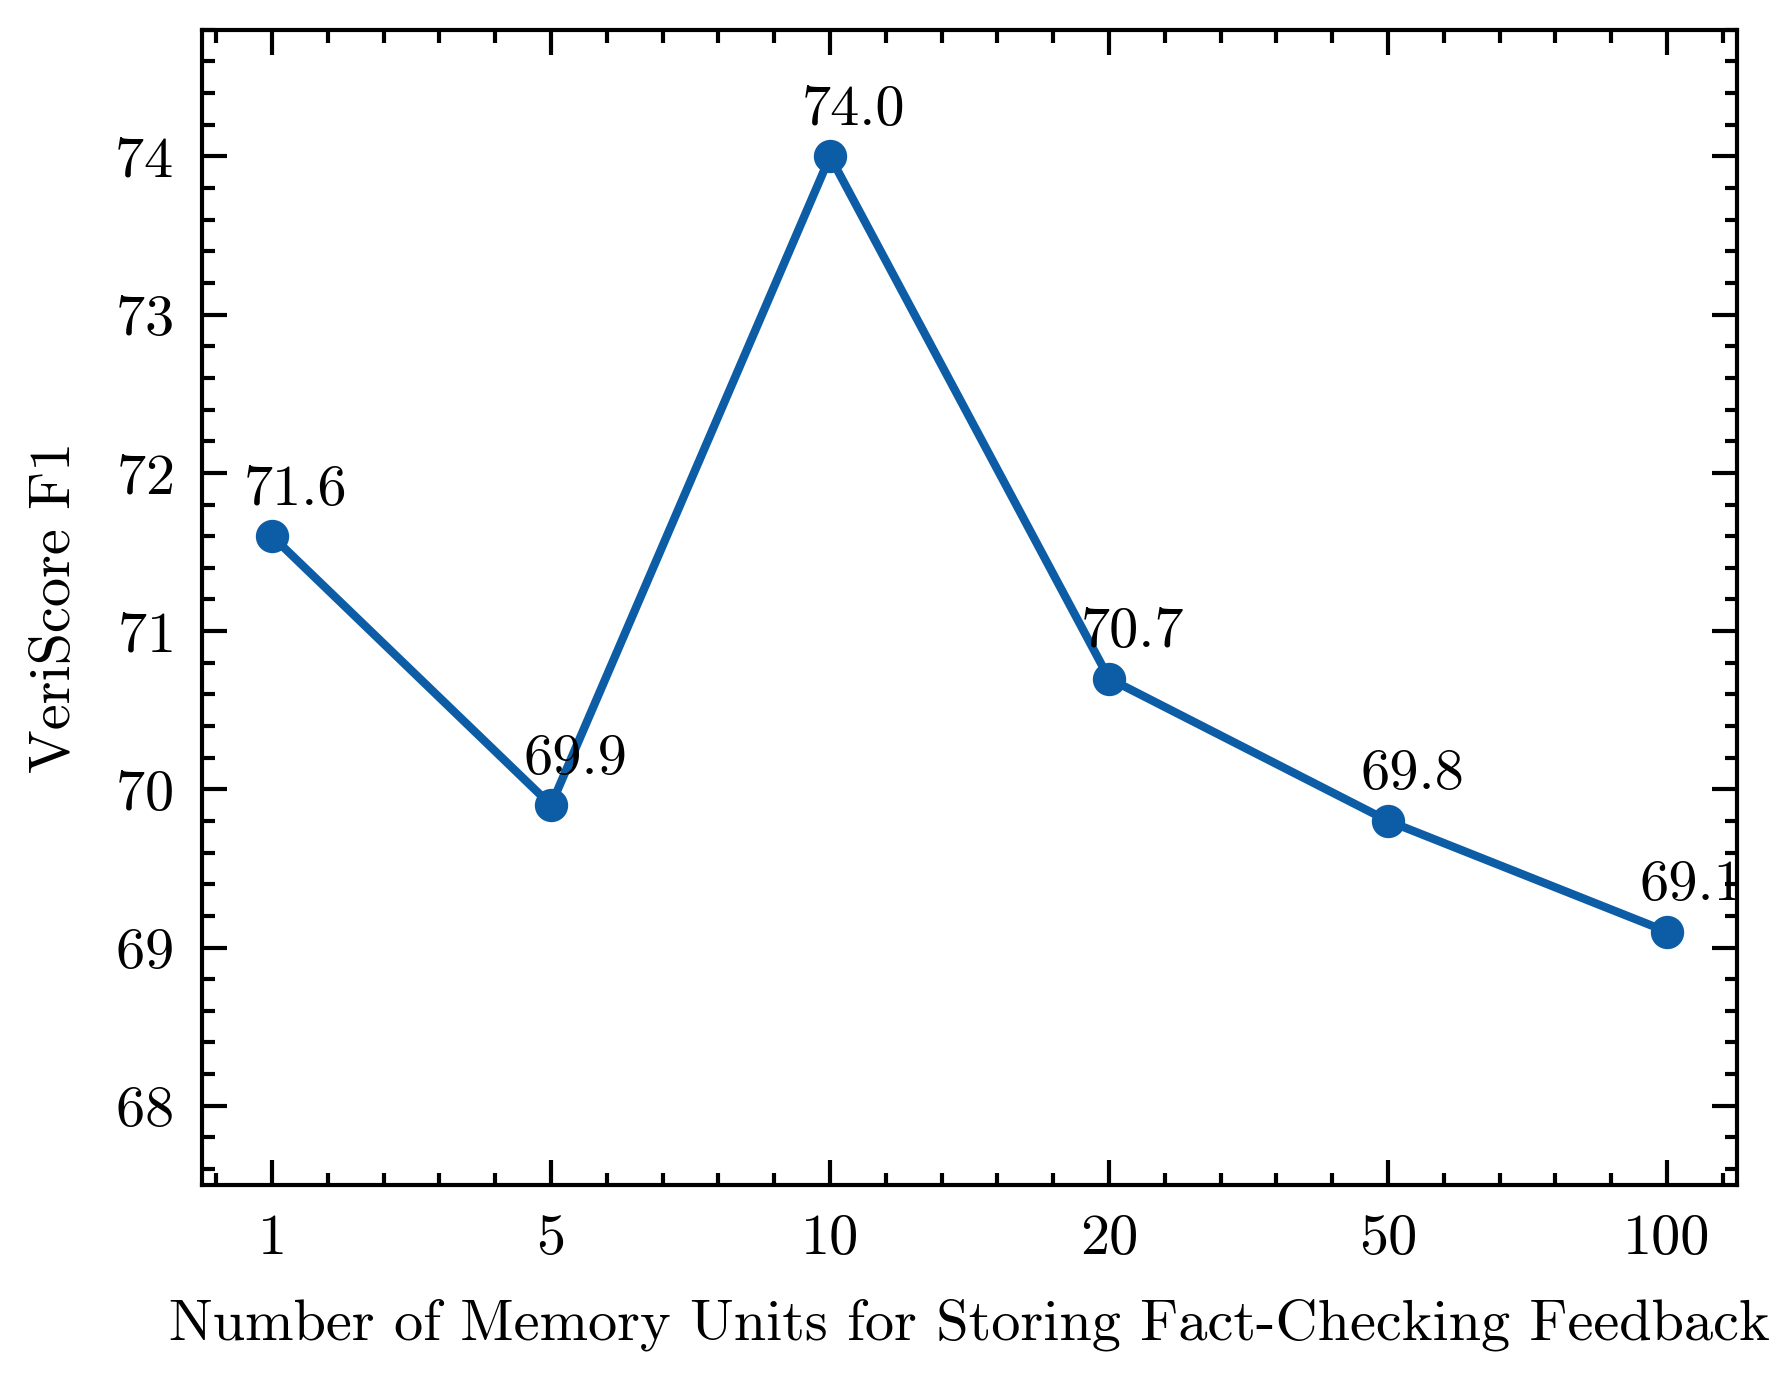
\includegraphics[width=0.4\textwidth]{figures/factcheck_memory_config_ablation.png}
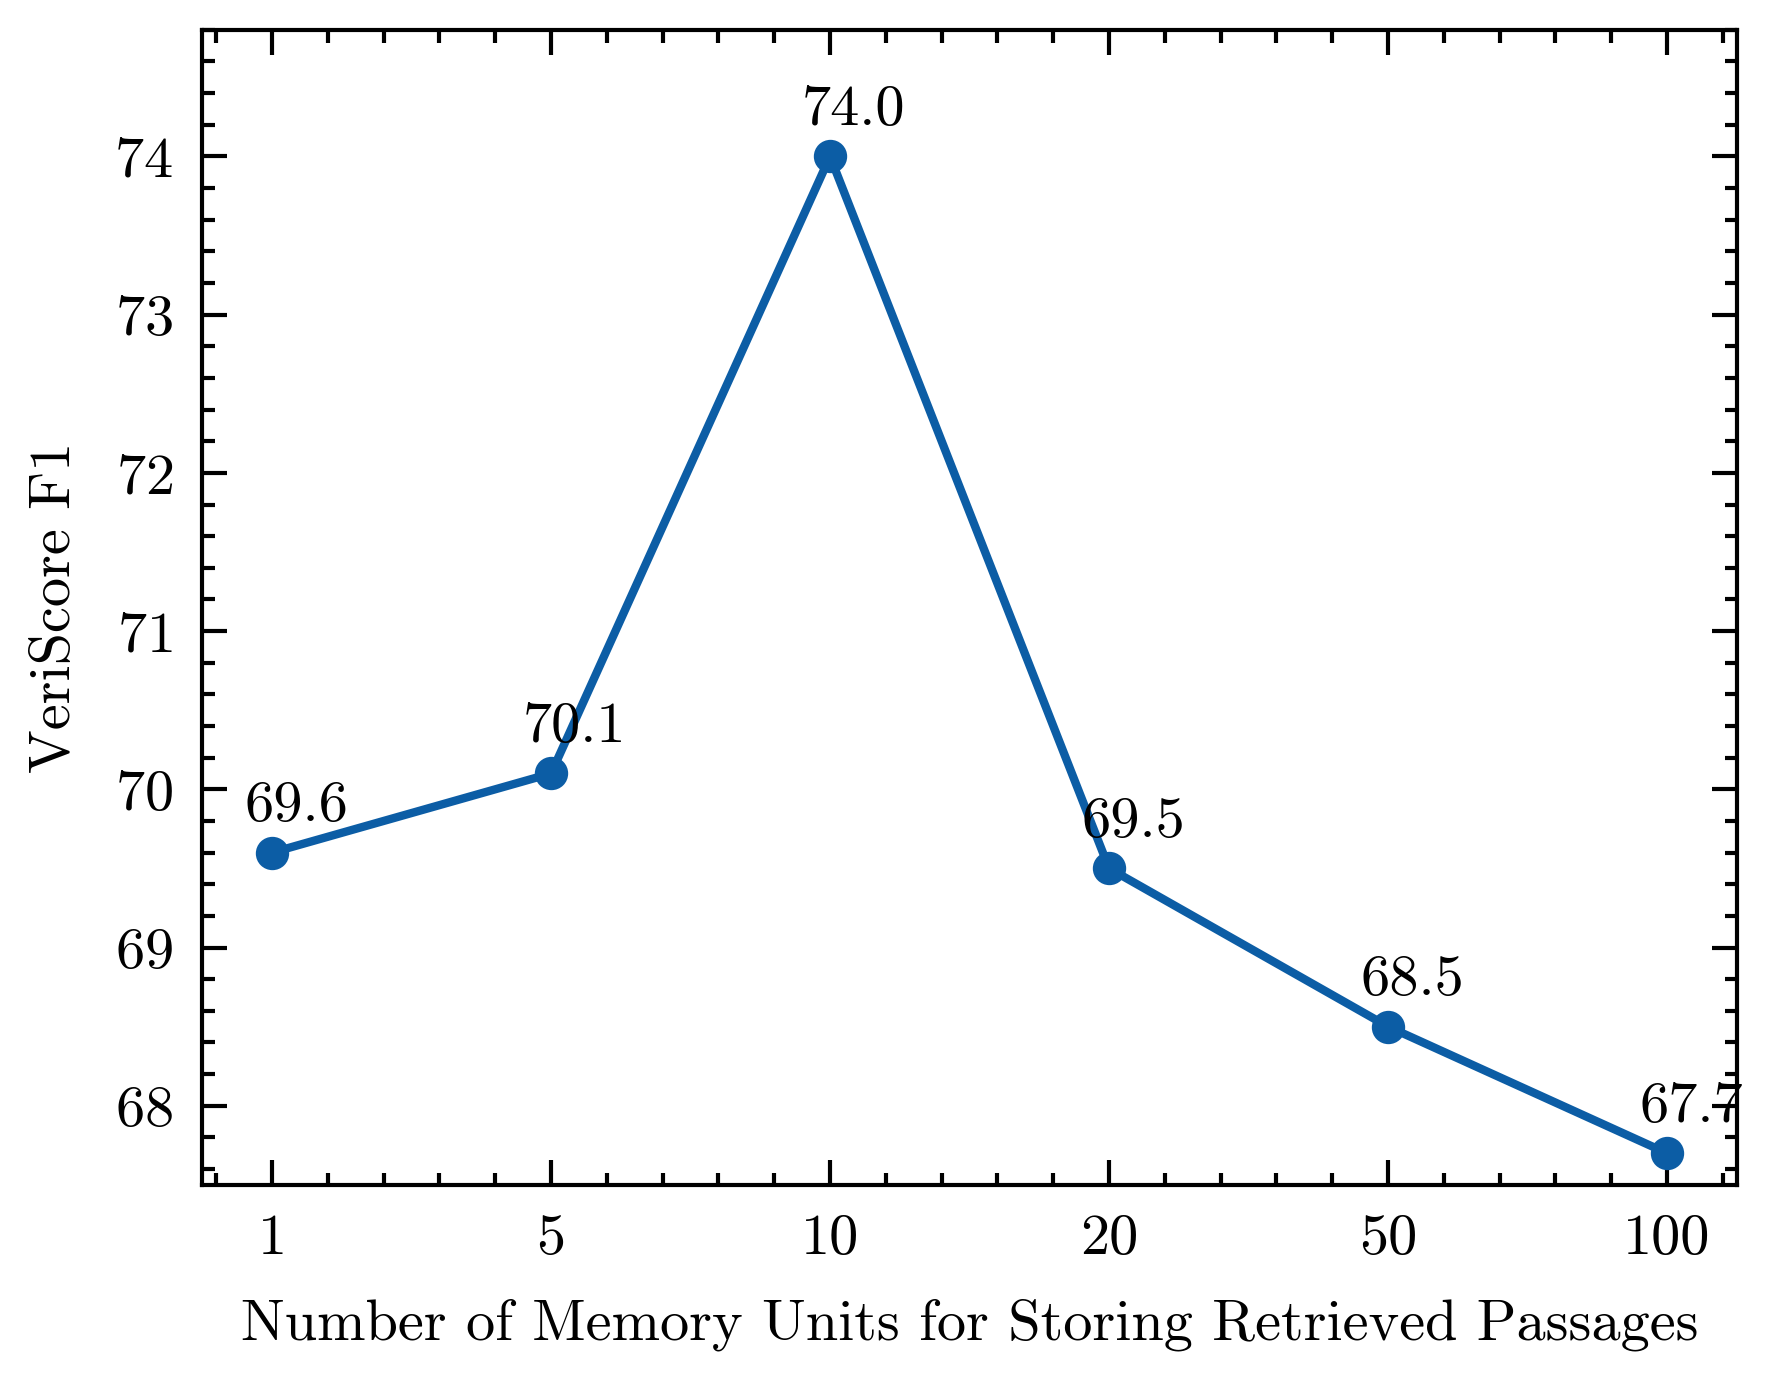
\includegraphics[width=0.4\textwidth]{figures/retrieval_memory_config_ablation.png}
    \caption{\vs F$_1$ over 50 prompts from \lf when varying number of memory units used for storing retrieved passages and fact-checking feedback. Each memory unit stores 128 tokens.}
    \label{fig:memory_unit_number_ablation}
\end{figure}

In Figure~\ref{fig:memory_unit_number_ablation}, we investigate how varying the numbers of memory units used for storing fact-checking feedback and retrieved passages may impact factuality. When adjusting the configuration for one, we keep the other constant to facilitate easier interpretation of the results. Overall, we observe that having a large amount of memory units for either fact-checking feedback or retrieved passages \textit{negatively} impacts factuality. 
This is likely because a significant amount of stale information remains in working memory for an extended period without being updated, as we adhere to the FIFO rule for updating working memory. 
Consequently, this information becomes outdated as the generation process continues.



\begin{table}
    \centering
    \begin{tabular}{lccc} \toprule
      Memory Shape ($M\times k$) & $128\times 20$ & $256\times 10$ & $512\times 4$ \\ \midrule
       F1  & \bf 74.0 & 69.0 & 68.2 \\\bottomrule
    \end{tabular}
    \caption{\vs F$_1$ over 50 prompts from \lf with different shapes of working memory. We allocate an equal number of memory units for both retrieval and fact-checking feedback.}
    \label{tab:memory_unit_shape_ablation}
\end{table}


In Table~\ref{tab:memory_unit_shape_ablation}, we examine the impact of varying memory unit shapes on factuality. To ensure a fair comparison, we maintained a consistent total number of tokens in working memory across different experimental setups. 
Notably, our findings suggest that models favor shorter, more memory units over longer, fewer ones. We hypothesize that this preference arises because 128 tokens approximately match the length of a retrieved passage, allowing the attention mechanism to effectively cover one individual passage at a time. 
In contrast, longer memory units combine multiple passages into a single unit, which may compel the attention to focus on less relevant passages when they are grouped with more relevant ones.



\subsection{Feedback Forms}




\begin{table}[t]
    \centering
    \begin{tabular}{cccccc} \toprule
         \multirow{2}{*}{\begin{minipage}{1.3in}Passages determining a claim is incorrect\end{minipage}} & \multirow{2}{*}{\begin{minipage}{1.3in}Passages determining a claim is correct\end{minipage}} & \multirow{2}{*}{\begin{minipage}{1.3in}Instructions\\for nonfactual claims\end{minipage}}   & Precision & Recall & F$_1$  \\
        & & & & & \\\midrule
         \checkmark & \checkmark & \checkmark &  77.3 & 64.0 & 66.8 \\
         \checkmark & & & 76.4 &\bf  67.4 & 67.9 \\
         & \checkmark & & 77.5 & 67.2 & \bf 69.4 \\
         & & \checkmark & 67.1 & 66.2 & 66.7 \\
         \checkmark & \checkmark &   &\bf  80.8 & 66.1 &\bf  69.3 \\
         & & & 72.5 & 65.9 &	66.2 \\\midrule
         \multicolumn{3}{r}{Llama-3.1$_{\text{70B}}$} & 65.8 &	67.1 &	65.5 \\
         \multicolumn{3}{r}{Llama-3.1$_{\text{70B}}$ + RA} & 70.1 & 66.1 & 65.9 \\ \bottomrule
    \end{tabular}
    \caption{Comparing different feedback forms for fact-checkers. We report \vs over 50 prompts from \lf.}
    \label{tab:feedback_form}
\end{table}


In this analysis, we explore various feedback formats utilized by fact-checkers. The models in \vs offers 2 types of information: a list of both factual and nonfactual claims, along with relevant passages that support these factual and nonfactual judgments. To examine the impact of these feedback formats, we conduct experiments using different combinations of these information types in the working memory. For the supporting passages, we combine them using new line symbols. For the list of claims, we apply an instruction template as follows to encode nonfactual claims:
\begin{TextBox}{}
{Please refrain from including the following imprecise statements: (1) nonfactual claim\textsubscript{1} (2) nonfactual claim\textsubscript{2} ...}
\end{TextBox}

Our results are shown in Table~\ref{tab:feedback_form}. Overall, fact-checking feedback is beneficial compared to the base model with and without retrieval augmentation. 
The specific types of feedback also play a crucial role. Incorporating all feedback forms does not enhance model performance, with supporting passages proving more effective than instructions. 
We notice that instructing models not to generate specific details often results in misunderstanding. Models might rephrase the instruction, include the nonfactual statement in their response, and then add a clarification indicating the previous statement is nonfactual, such as ``\textit{(Note: This is a nonfactual claim and may not be accurate.)}''. We leave a better design of feedback forms to future work. 
Interestingly, when we exclude all the textual feedback from fact-checkers and only pause and regenerate in the presence of nonfactual sentences, performance still slightly improves.


\subsection{Model Confidence}




One important question remains is when to refresh the working memory. To study it, we conducted a comparative analysis of different criteria for refreshing working memory and regeneration. 
Since the working memory consists of the retrieval memory and fact-checking memory, which can have interacting effects, we first investigate when to trigger the retriever alone (without fact-checking memory) and then investigate when to trigger the fact-checker (when retrieval interval $T_r$ is set to 1).

\paragraph{Fixed intervals for refreshing working memory}
As shown in Figure~\ref{fig:interval-fixed}, when using a fixed retrieval interval, an intermediate interval seems to perform well. 
This may be due to the fact that overly frequent retrieval can add irrelevant and conflicting information to the memory. 
With fact-checking feedback in memory, it seems frequent verification and regeneration is not always beneficial due to the fact that we only regenerate once and the regenerated sentence is not always better.

\paragraph{Model confidence for refreshing working memory}
In practice, fixed retrieval and verification intervals may be unnecessary and lead to sub-optimal performance. We explore whether model-confidence can serve as a signal for refreshing working memory. Specifically, we compare two different metrics for model confidence: (1) \textbf{Entropy}: average entropy of generated tokens in a sentence, and (2) \textbf{Min-prob}: minimum probability of tokens in a sentence. A higher threshold for entropy results in less frequent memory update, and a higher threshold for min-prob results in more frequent memory update. 
Since external fact-checkers can be computationally expensive, we first examine if we can use model confidence as a signal for retrieval and regeneration, without using an auxiliary fact-checking model to provide feedback. 
As shown in Figure~\ref{fig:interval-entropy} and \ref{fig:interval-prob} (blue line), we observe empirically intermediate thresholds for retrieval perform well, leading to to better F$_1$ when compared to the settings in Figure~\ref{fig:interval-fixed}, where we use different fixed intervals for retrieval. 
With external fact-checkers, we investigate if we can use model confidence as a signal to trigger verification and regeneration to improve generation efficiency. 
In Figure~\ref{fig:interval-entropy} and \ref{fig:interval-prob} (red line), when chosen at an appropriate threshold, both entropy and min-prob can outperform the baseline (using fixed verification interval $T_v=8$) despite with less frequent verification.



\begin{figure}[t!]
\centering
\begin{subfigure}[t]{0.32\textwidth}
        \centering
        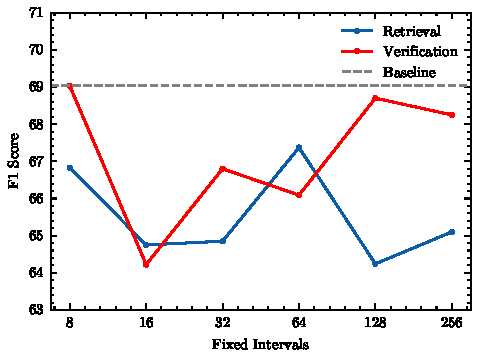
\includegraphics[width=\textwidth]{figures/fixed_interval.pdf}
        \caption{\vs F$_1$ when using fixed retrieval and verification intervals.}
        \label{fig:interval-fixed}

    \end{subfigure}%
    \hfill
    \begin{subfigure}[t]{0.32\textwidth}
        \centering
            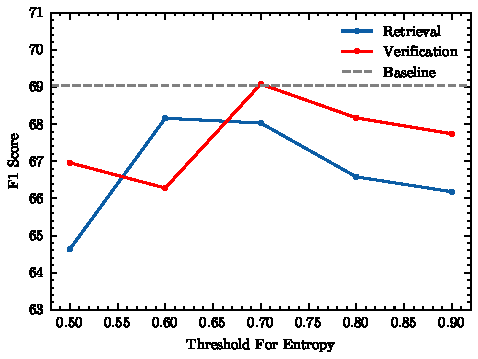
\includegraphics[width=\textwidth]{figures/entropy_threshold.pdf}
        \caption{F$_1$ when using entropy thresholds for triggering retrieval and verification.}
                \label{fig:interval-entropy}

    \end{subfigure}
    \hfill
    \begin{subfigure}[t]{0.32\textwidth}
        \centering
            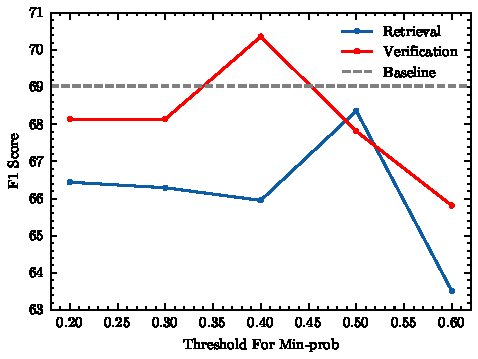
\includegraphics[width=\textwidth]{figures/prob_threshold.pdf}
        \caption{F$_1$ when using min-prob thresholds for triggering retrieval and verification.}
            \label{fig:interval-prob}

    \end{subfigure}
\caption{Comparison of different criteria for refreshing working memory over 50 prompts from \lf. The baseline uses retrieval interval $T_r = 1$ and verification interval $T_v = 8$.}
\label{fig:interval}
\end{figure}


\subsection{Knowledge from Retrieval}

\begin{table}[t!]
    \centering
    \begin{tabular}{lcccc} \toprule
       Datastore  & \lf & \bio & \alpaca & \fava \\\midrule
       Wiki  & 63.0 & 39.1 & 55.4 & 50.5 \\
       C4 & 66.8 & \bf 45.4 & 58.6 & 53.6 \\
       C4 + Wiki & \bf 69.0 & 43.8 & \bf 58.8 & \bf 54.6 \\ \bottomrule
    \end{tabular}
    \caption{\vs F$_1$ over 50 prompts from \lf, \alpaca, \fava and \bio with different retrieval datastores.}
    \label{tab:retrieval_corpus_ablation}
\end{table}


We present the results of using different retrieval corpora in Table~\ref{tab:retrieval_corpus_ablation}, including Wikipedia, C4, or both of them together.
Likely due to its broader coverage, C4 is more effective than Wikipedia in helping the model produce more factual responses. 
Combining C4 with Wikipedia further enhances the factual accuracy (except for \bio), probably because they offer complementary sets of knowledge.










